\documentclass{article}
\usepackage[utf8]{inputenc}
\usepackage{amsmath}
\usepackage{listings}
\usepackage{color}
\usepackage{graphicx}
\usepackage[margin=1in]{geometry}
\usepackage{hyperref}
\usepackage{gensymb}
\graphicspath{ {} }

\definecolor{dkgreen}{rgb}{0,0.6,0}
\definecolor{gray}{rgb}{0.5,0.5,0.5}
\definecolor{mauve}{rgb}{0.58,0,0.82}

%\lstset{frame=tb,
%  language=c,
%  aboveskip=3mm,
%  belowskip=3mm,
%  showstringspaces=false,
%  columns=flexible,
%  basicstyle={\small\ttfamily},
%  numbers=left,
%  numberstyle=\tiny\color{gray},
%  keywordstyle=\color{blue},
%  commentstyle=\color{dkgreen},
%  stringstyle=\color{mauve},
%  breaklines=true,  
%  breakatwhitespace=true,
%  tabsize=2
%}



\lstset{
  language=C,                % choose the language of the code
  numbers=left,                   % where to put the line-numbers
  stepnumber=1,                   % the step between two line-numbers.        
  numbersep=15pt,                  % how far the line-numbers are from the code
  backgroundcolor=\color{white},  % choose the background color. You must add \usepackage{color}
  showspaces=false,               % show spaces adding particular underscores
  showstringspaces=false,         % underline spaces within strings
  showtabs=false,                 % show tabs within strings adding particular underscores
  tabsize=4,                      % sets default tabsize to 2 spaces
  captionpos=b,                   % sets the caption-position to bottom
  breaklines=true,                % sets automatic line breaking
  breakatwhitespace=true,         % sets if automatic breaks should only happen at whitespace
  title=\lstname,                 % show the filename of files included with \lstinputlisting;
    aboveskip=1mm,
  belowskip=1mm,
   basicstyle={\ttfamily},
}


\title{\textbf{Pellet Smoker Operation}\\ Biomass Controls, LLC  \\ \today}
\author{David Paquette, Michael Paquette \\\\Customer: Myron Mixon Smokers}
\date{}

\begin{document}

\maketitle
\tableofcontents
\section{Pellet Smoker Overview}
\subsection{Design Requirements}
\begin{itemize}  
\item Transition from stand-by, start-up, smoke, cook, and hold states 
\item Maintain temperatures in the range of 150\degree F  to 350\degree F with an allowable error of 10\degree F peak-to-peak.
\item Produce varying levels of smoke, defined by user
\end{itemize}
\section{State Logic}
\begin{center}
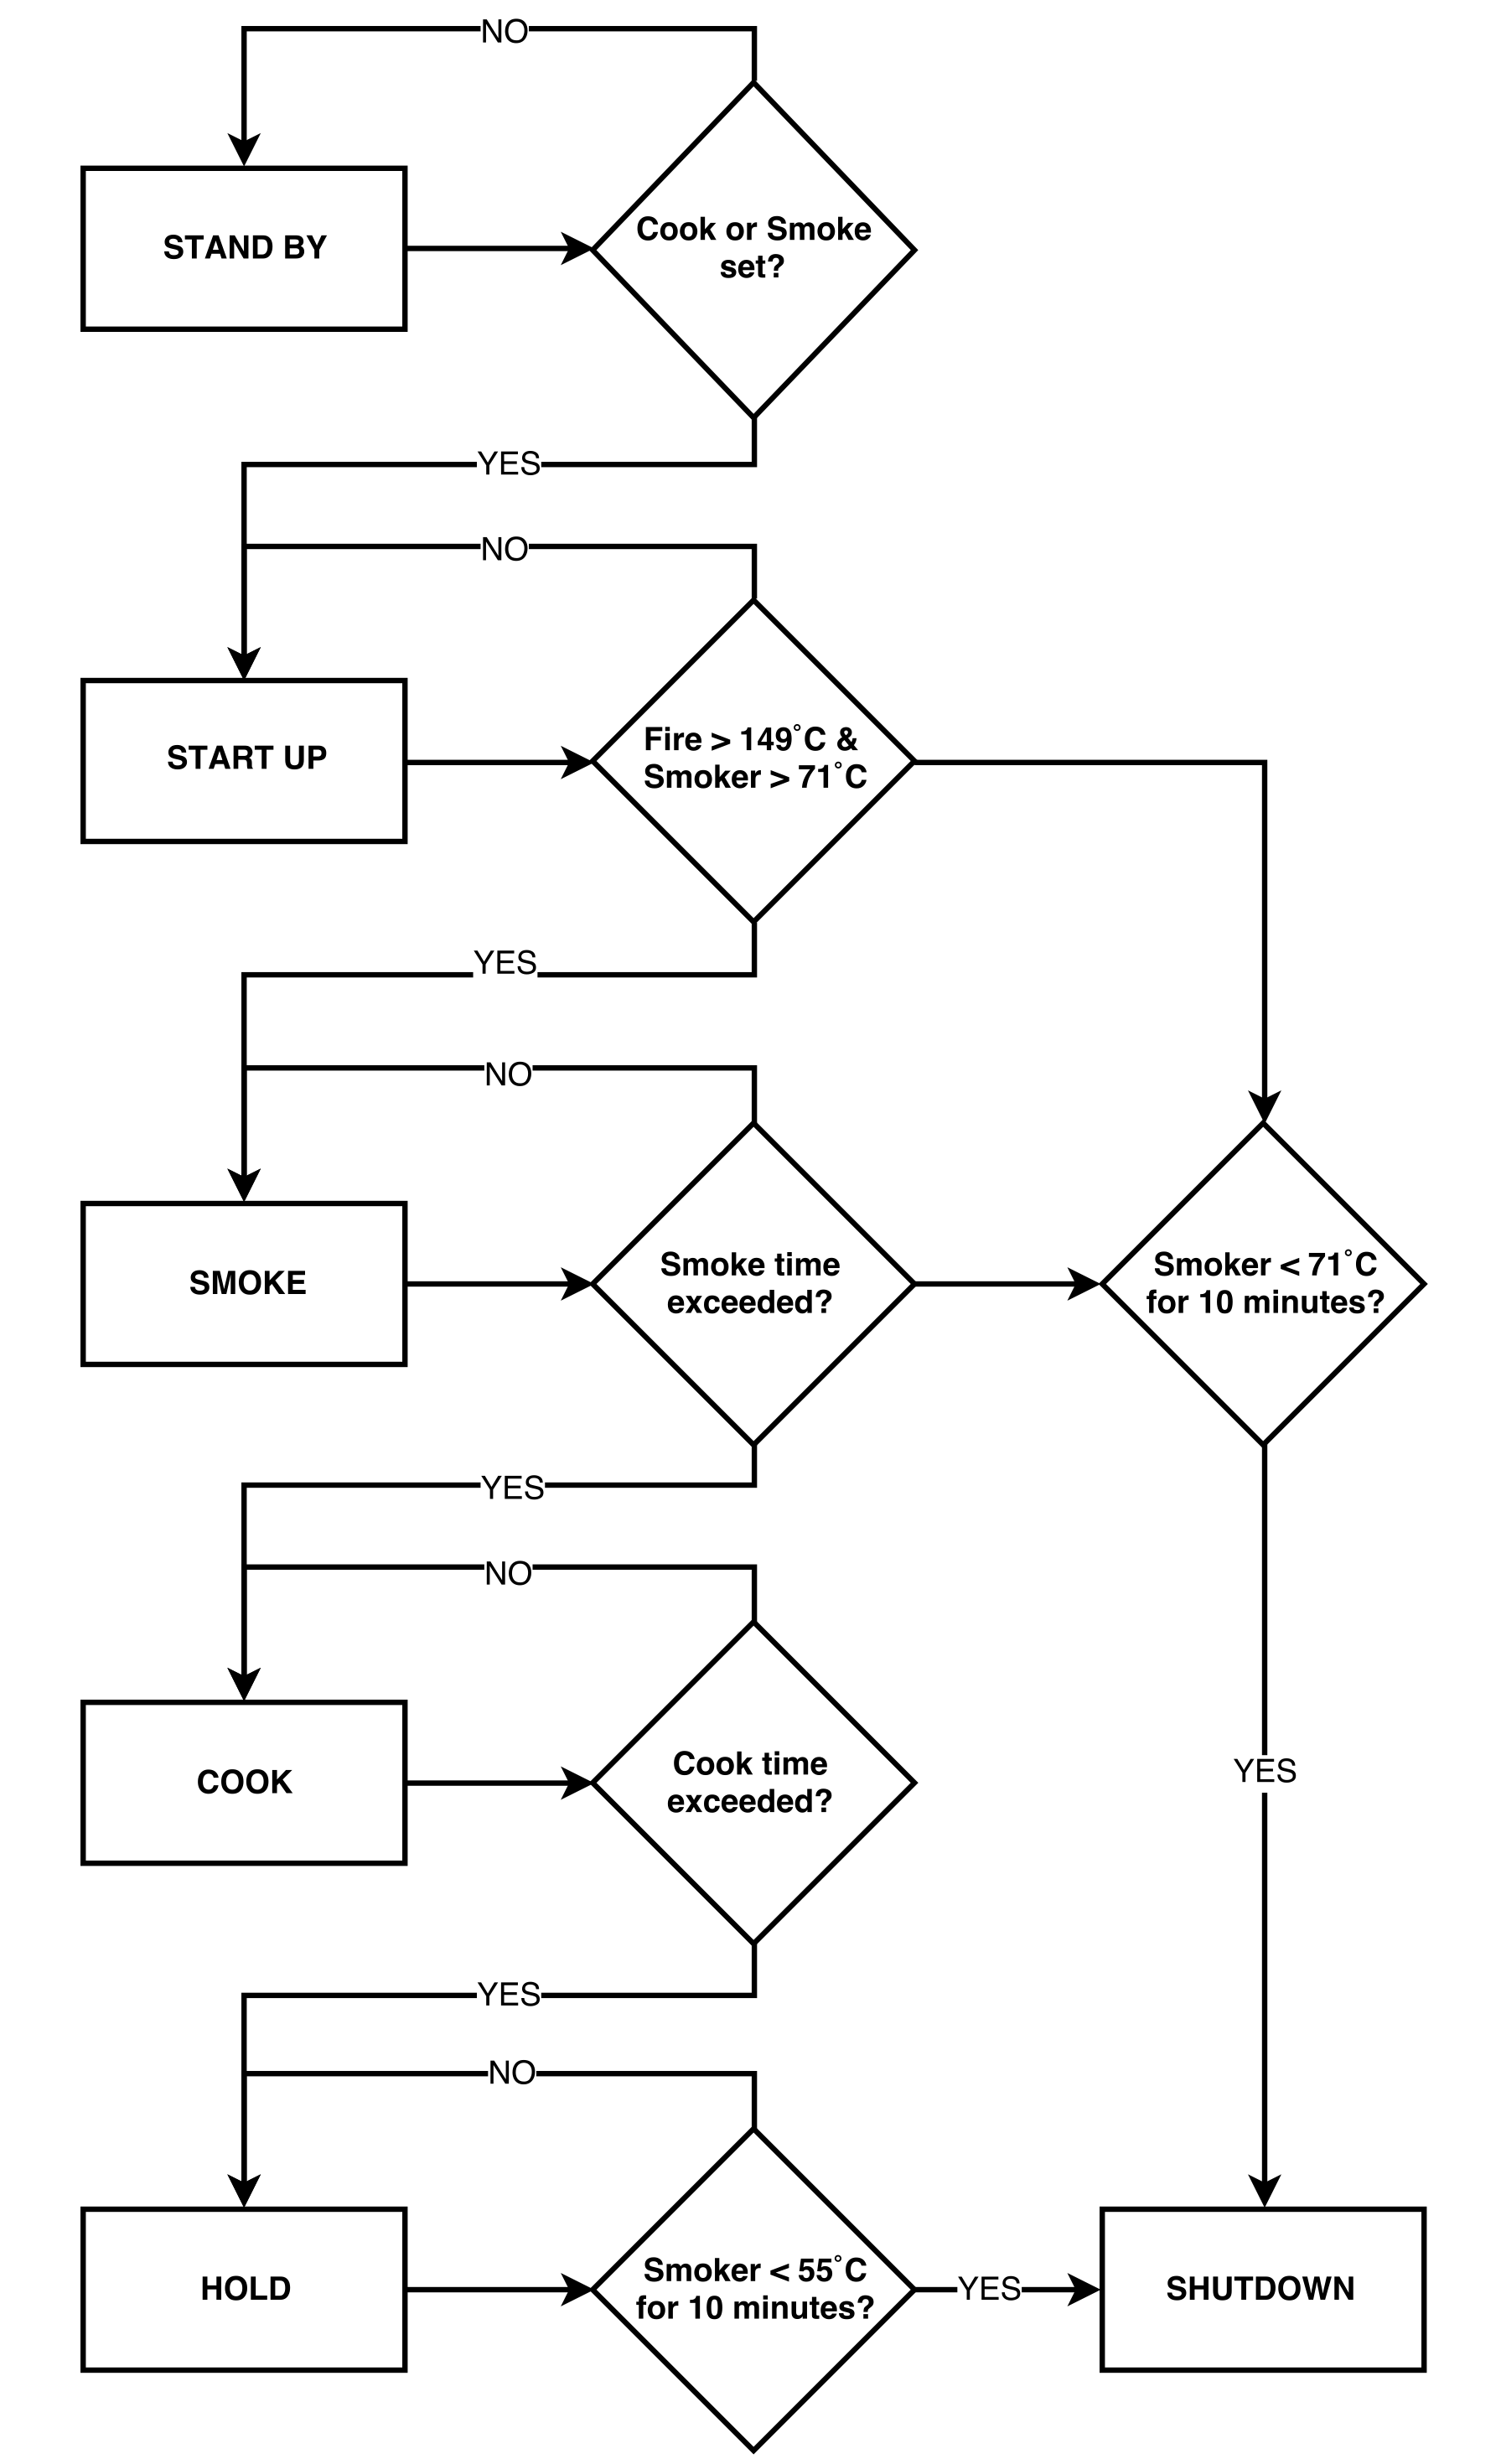
\includegraphics[scale=.5]{stateTransition}
\centering
\end{center}
\textbf{FIG1.} State transition diagram overview.
\subsection{Stand By State}
Wait until a user enters the amount of time they want to smoke and cook their food. When they enter a time we transition to start up.
\subsection{Start Up State}
In this state our goal is to reach the minimum cooking temperature of 150\degree F. When we reach this temperature and both our fire temperatures are reasonable, we move to smoke state. Upon entering this state, we turn the igniters on and wait for 3 minutes. We run at a constant auger duty cycle of 33.3\% with a period of 90 seconds and a constant fan duty cycle of 100\%. When our either fire temperature exceeds 149\degree C the auger duty cycle changes to 2.0\% with a period of 100 seconds. During this state the igniters are on when fire temperatures are below 149 \degree C.  
\subsection{Smoke State}
Here we maintain a user selectable smoker temperature. We leave when we have smoked for the set amount of smoke time, specified by the user. The fan duty cycle is set to the auger duty cycle.
\subsection*{Cook State}
Here we maintain a user selectable smoker temperature. That's really it. We leave when we have cooked for the set amount of cook time, specified by the user.
\subsection{Hold State}
Here we maintain a user selectable hold temperature indefinitely.
\subsection{Shutdown State}
Auger stays off, igniter stays off. We turn the fan on to remove any excess fuel.
\section{Process Control}
\subsection{Overview}
In the temperature controlled states (Cook, Smoke, Hold) we use the control architecture outlined in figure 2. As shown, the auger's duty cycle is controlled by a PI controller. The fan is controlled by using an open loop ratio control scheme.
\begin{center}
\includegraphics[scale=.15]{blockdiag}
\centering
\end{center}
\textbf{FIG2.} Control architecture.

\subsection{Auger Control}
We are using standard PI feedback to modulate the duty cycle of the auger. Because the auger is not a PWM modulated actuator, but is using simple on/off relay control, we have to use relay on/off time. We are keeping the on time of the augers constant at 15 seconds, which is a standard on time we found across a wide range of pellet grills.  \\ \\ As shown in figure 2, the PI controller outputs a duty cycle value. Because we know the auger's on time ($t_{on}$) and the duty cycle ($D$) is provided by the controller, we compute our auger off time ($t_{off}$) by first computing the period ($T$) using
\[ T = \frac{t_{on} \times 100}{D}\]
And then we use 
\[ t_{off} = T-t_{on}\]
to compute of auger's off time. We use $t_{off}$, $T$, $t_{on}$ to translate the controller output ($D$) to our final controller element's relay on/off time. This is just pulse density modulation (PDM).

\subsubsection{Notes On the PI Controller}
We are using the non-interactive PI control algorithm, which is described by
\[ CO = K_C\left(e(t)+\frac{1}{T_I}\int e(t)dt \right)\]
Where $K_C$ is our controller gain, $CO$ is our controller output and $T_I$ is our integral time (sometimes referred to as our reset time) and $e(t)$ is our process variable set point ($SP$) minus process variable ($PV$) or $e(t) = SP-PV$.
Our integral gain would then be $K_I=K_C/T_I$. To implement this on a digital controller we use
\[ CO[n+1] = K_C\left(e[n]+\frac{T_s}{T_I}\sum_{n} e[n] \right)\]

Where $T_S$ is our sampling period, which we have set to 5 seconds or $f_s=0.2$ Hz, or one sample per 5 seconds. To improve over shoot we are going to need to implement and tune a full PID controller (right now we are only using a PI controller). The derivative term should help stabilize the response during start up and set point changes.
\subsubsection{System Identification}
We are required to find 2 parameters that dictate the behavior of our controller, $K_C$ and $T_I$. To tune these values we followed the standard step response test. The $PV$ was brought to a steady state value of 122\degree C using a $CO$ of 4.44\%. We changed our $CO$ to 10\%, which resulted in a $PV$ of 149\degree C. To find our process gain $K_p$ we used

\[K_p = \frac{\Delta PV}{\Delta CO}\]

Which resulted in

\[ K_p = \frac{149-122}{10-4.44}=4.865\]

By inspecting the response our process dead time was $\theta_p = 120$ seconds and our process time constant $T_p = 1200$ seconds. This approximates our system as the first order linear differential equation with dead time as
\[ 1200\cdot \frac{dT_{sm}(t)}{dt}+T_{sm}(t)=4.865\cdot D_{ag}(t)\cdot u(t-120)\]
or (in the Laplace domain)
\[ G(s) = \frac{T_{sm}(s)}{D_{ag}(s)} = e^{-120s}\frac{4.865}{1200s+1}\]

Where $T_{sm}$ is the temperature of the smoker, and $D_{ag}$ is the duty cycle of the auger.
\subsubsection{Gain Tuning}
Using the model we derived from testing we can use $K_p$, $T_p$ and $\theta_p$ to tune our PI controller. Because we are looking for a faster response time we decided on using the standard Cohen-Coon tuning rules (instead of the more robust IMC or lambda tuning) where
\[ K_C = \frac{0.9}{SM \times K_p} \times \left( \frac{T_p}{\theta_p}+0.092 \right) \]

\[ T_I = 3.33\theta_p \times \left(\frac{T_p+0.092\theta_p}{T_p+2.22\theta_p}\right)\]

Where $SM$ is our desired stability margin of 3.0. Using our process values we arrive with 
\[ K_C = 0.82885\]
\[ T_I = 354.175\]
Due to our model not being extremely accurate we round these values to
\[ K_C = 0.83\]
\[ T_I = 355\]
\subsection{Fan Control}
The fan we are using is also on/off relay controlled. It supplies anywhere from 40 to 90 $\frac{ft^3}{min}$. We were told the fan introduces oxygen into the burn process and something called the air-fuel ratio ($AFR$) is important to maintain. Because we are not measuring fuel or air flow, and cannot fully control air flow due to the final control element, the best we can achieve is open loop control of the $AFR$. 
\subsubsection{Air-Fuel Ratio Control}
First we need to relate the method of controlling the air flow to the method of controlling the fuel flow. We used the following mass-flow differential equation
\[ D_{fan}\cdot\frac{dV_{fan}}{dt}\cdot \rho_{air}=AFR_{mass} \cdot D_{auger}\cdot \frac{dm_{auger}}{dt}-\frac{dm_{ambient}}{dt}\]
Where $D_{fan}$ is the duty cycle of the fan, $V_{fan}$ is the speed of the fan, $\rho_{air}$ is the density of air, $D_{auger}$ is the duty cycle of the auger, $m_{auger}$ is the mass delivered by the auger and $m_{ambient}$ is the flow of mass delivered when the fan is off. We need to scale the $AFR_{mass}$ to use $D_{auger}$ and $D_{fan}$ using
\[ AFR_{mass} = \frac{\frac{dm_{air}}{dt}}{\frac{dm_{fuel}}{dt}} \]
and
\[ AFR_{scaled} = \frac{D_{air}}{D_{auger}} \]
The final mass flow equation results in
\[ AFR_{scaled} = \frac{D_{air}}{D_{auger}} = \frac{\frac{dm_{auger}}{dt}}{\frac{dV_{fan}}{dt}\times\rho_{air}}\times AF_{mass}\]
Using the following approximations
\[ AFR_{mass} = 16:1\]
\[ \frac{dm_{auger}}{dt} = 0.2 \frac{lbm}{min}\]
\[ \frac{dV_{fan}}{dt} = 70 \frac{ft^3}{min}\]
\[ \rho_{air} = 0.06243 \frac{lbm}{ft^3}\]
We can compute our $AFR_{scaled}$ using
\[ AFR_{scaled} = 16\times\frac{0.2}{70\cdot 0.06243} = 0.732\]
This means that when our duty cycle of the auger is set to $D_{auger}$ our duty cycle of our fan for a 16:1 air-fuel ratio is
\[ D_{fan}=0.732\times D_{auger}\]
So when our PI controller computes its $CO$, we set $D_{fan}$ to $0.732\times CO$. A more detailed control architecture is shown below

\subsection{Validation}
As shown below in figure 3 we are able to maintain our set point within the $\pm$ 5\degree F bounds. Over the course of this particular burn we stayed within the allowable range 92\% of the time (up from the first run of only 80\%).

\begin{center}
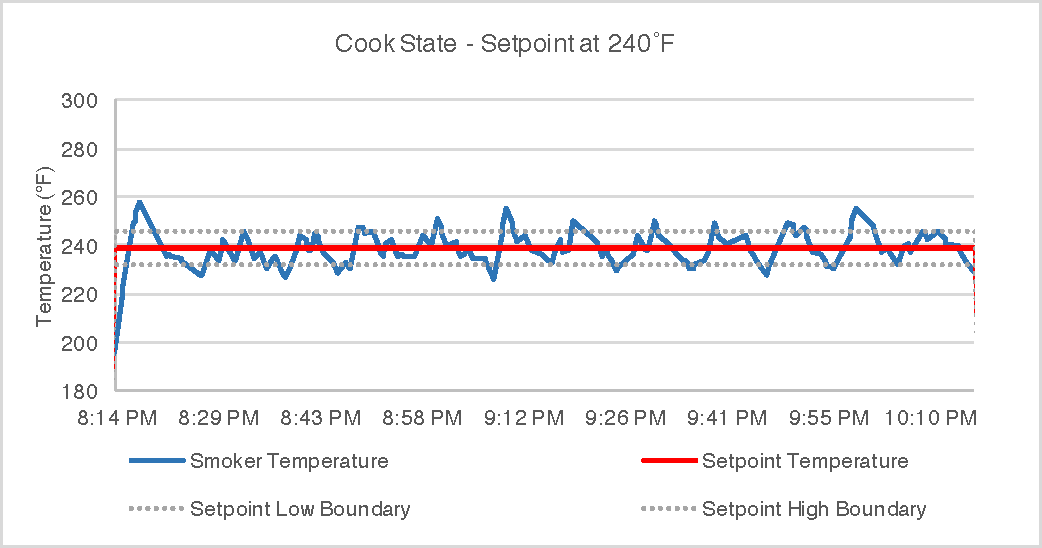
\includegraphics[scale=.95]{temphold}
\centering
\end{center}
\textbf{FIG3.} Plot of smoker temperature maintaining 240\degree F set point over 2 hours (second test). 

\begin{center}
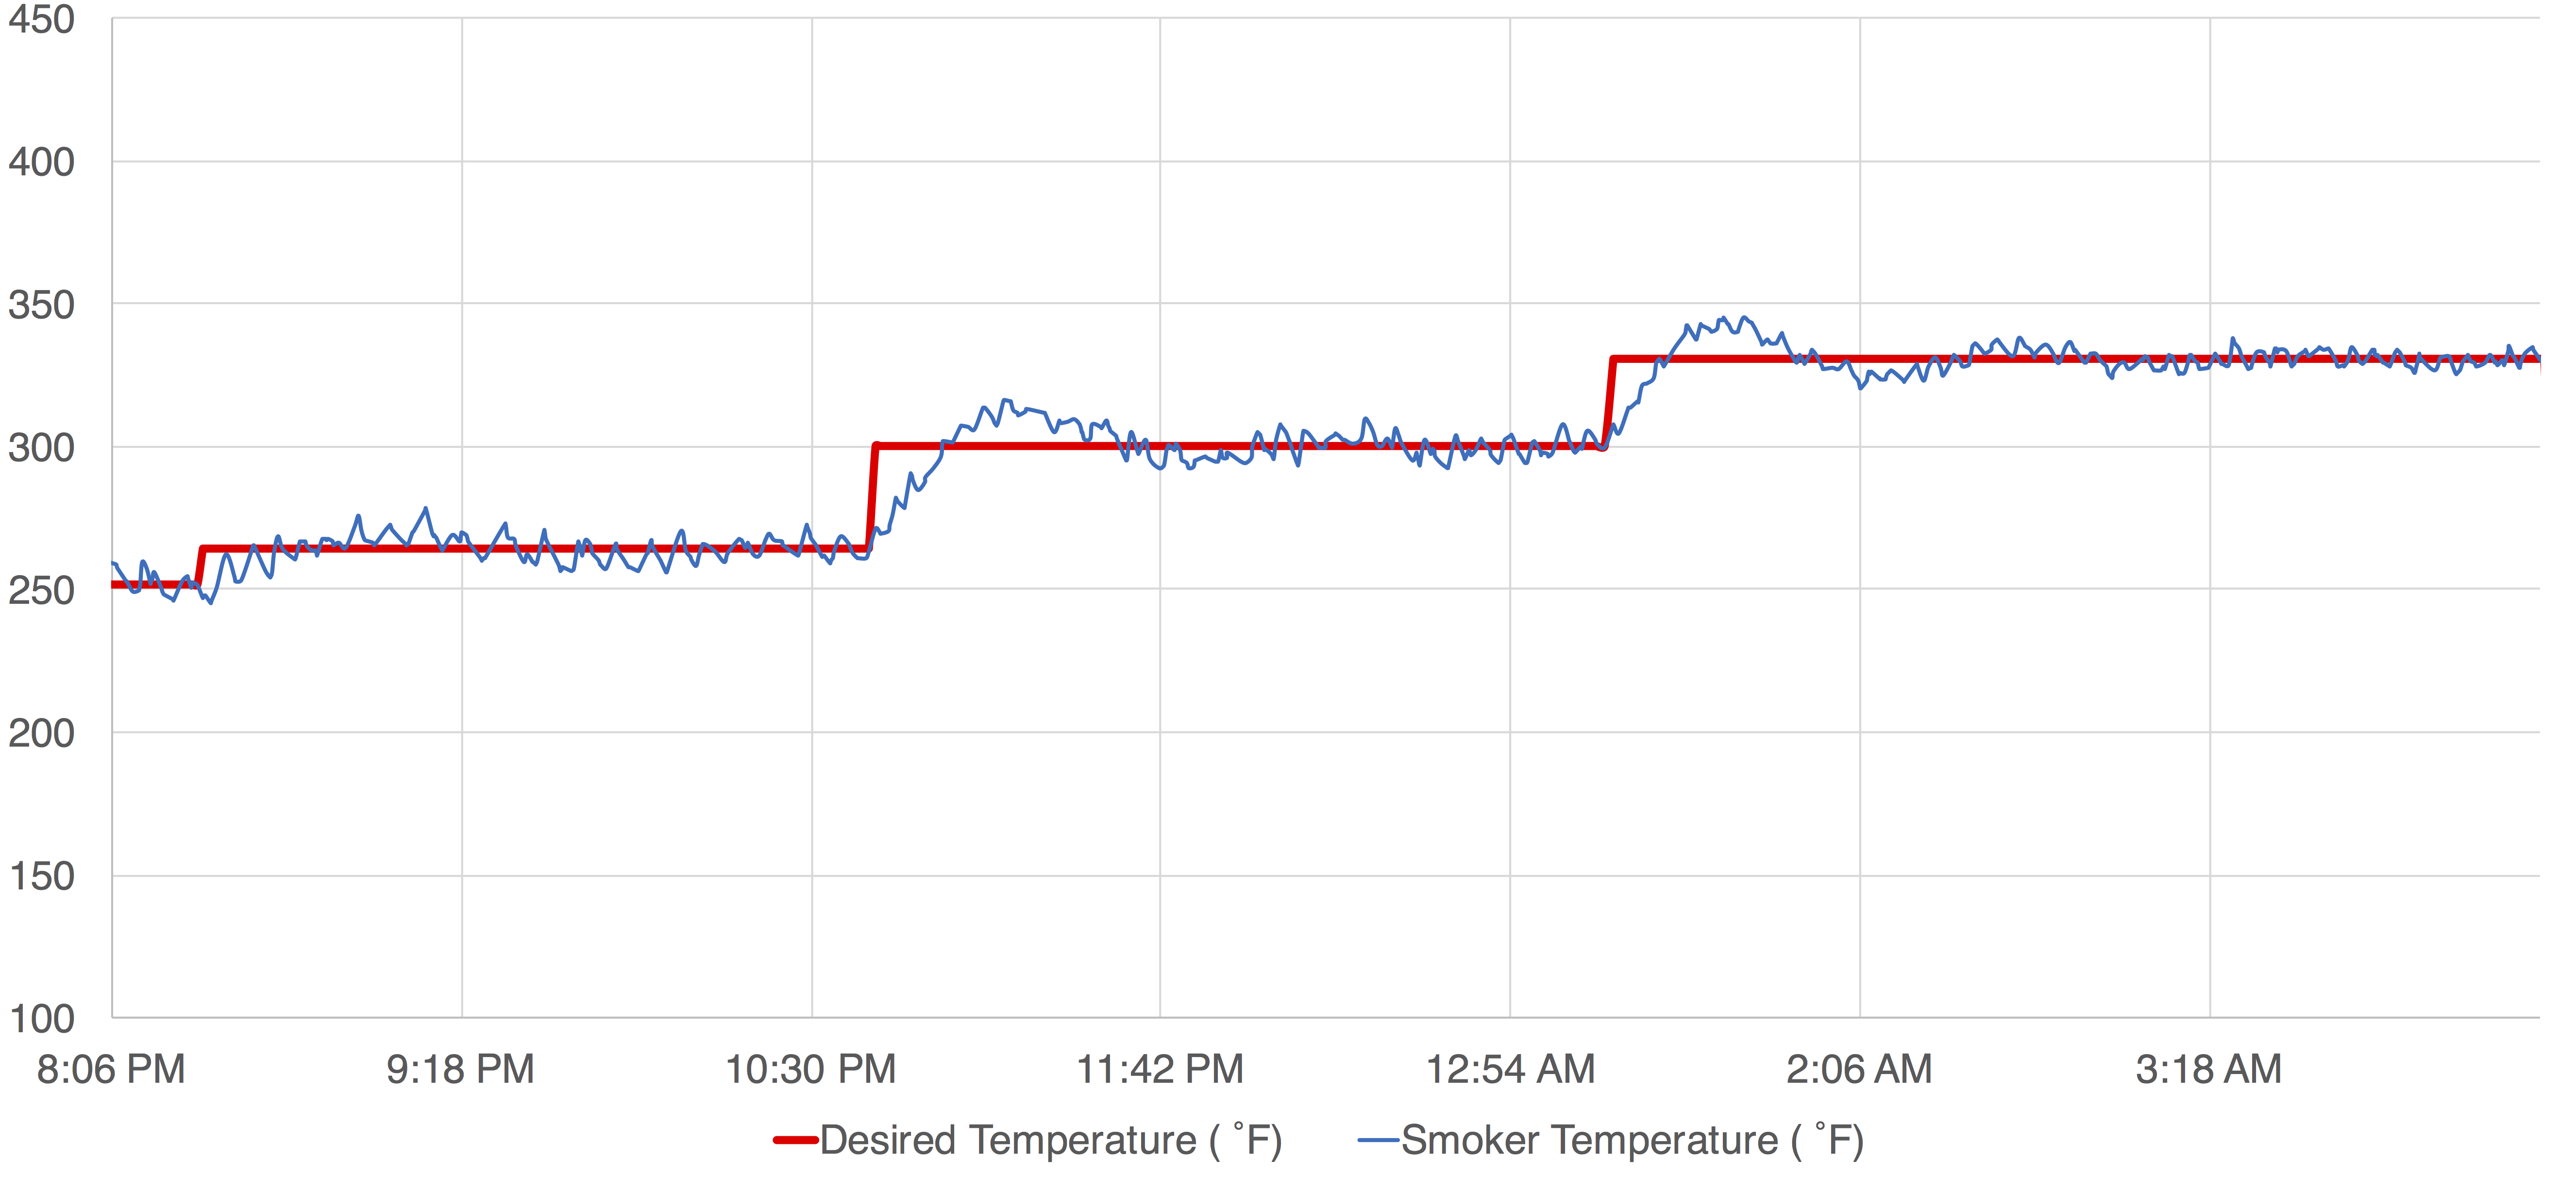
\includegraphics[scale=.37]{responses}
\centering
\end{center}
\textbf{FIG4.} Plot of set point tracking. Max overshoot is shown to be around 10\degree F to 15 \degree F. 
\\\\
Figure 4 shows the smoker responding to set point changes. The smoker temperature set point was changed 3 times. First from 250 \degree F to 264 \degree F, then from 264 \degree F to 300 \degree F, then finally from 300 \degree F to 330 \degree F. The controller handles the change just as designed (not too aggressive but with small overshoot). To reduce this over shoot, while maintaining the robustness of our controller, we will need to implement a full PID controller. Adding the derivative term will drastically speed up our response, decreasing settling time and overshoot. This was initially avoided because of the time constraint of only a 5 day testing period, adding an entirely new parameter ($T_D$) would have added much more complexity to the design. But to reduce overshoot/speed up our response we will most likely need it.
\begin{center}
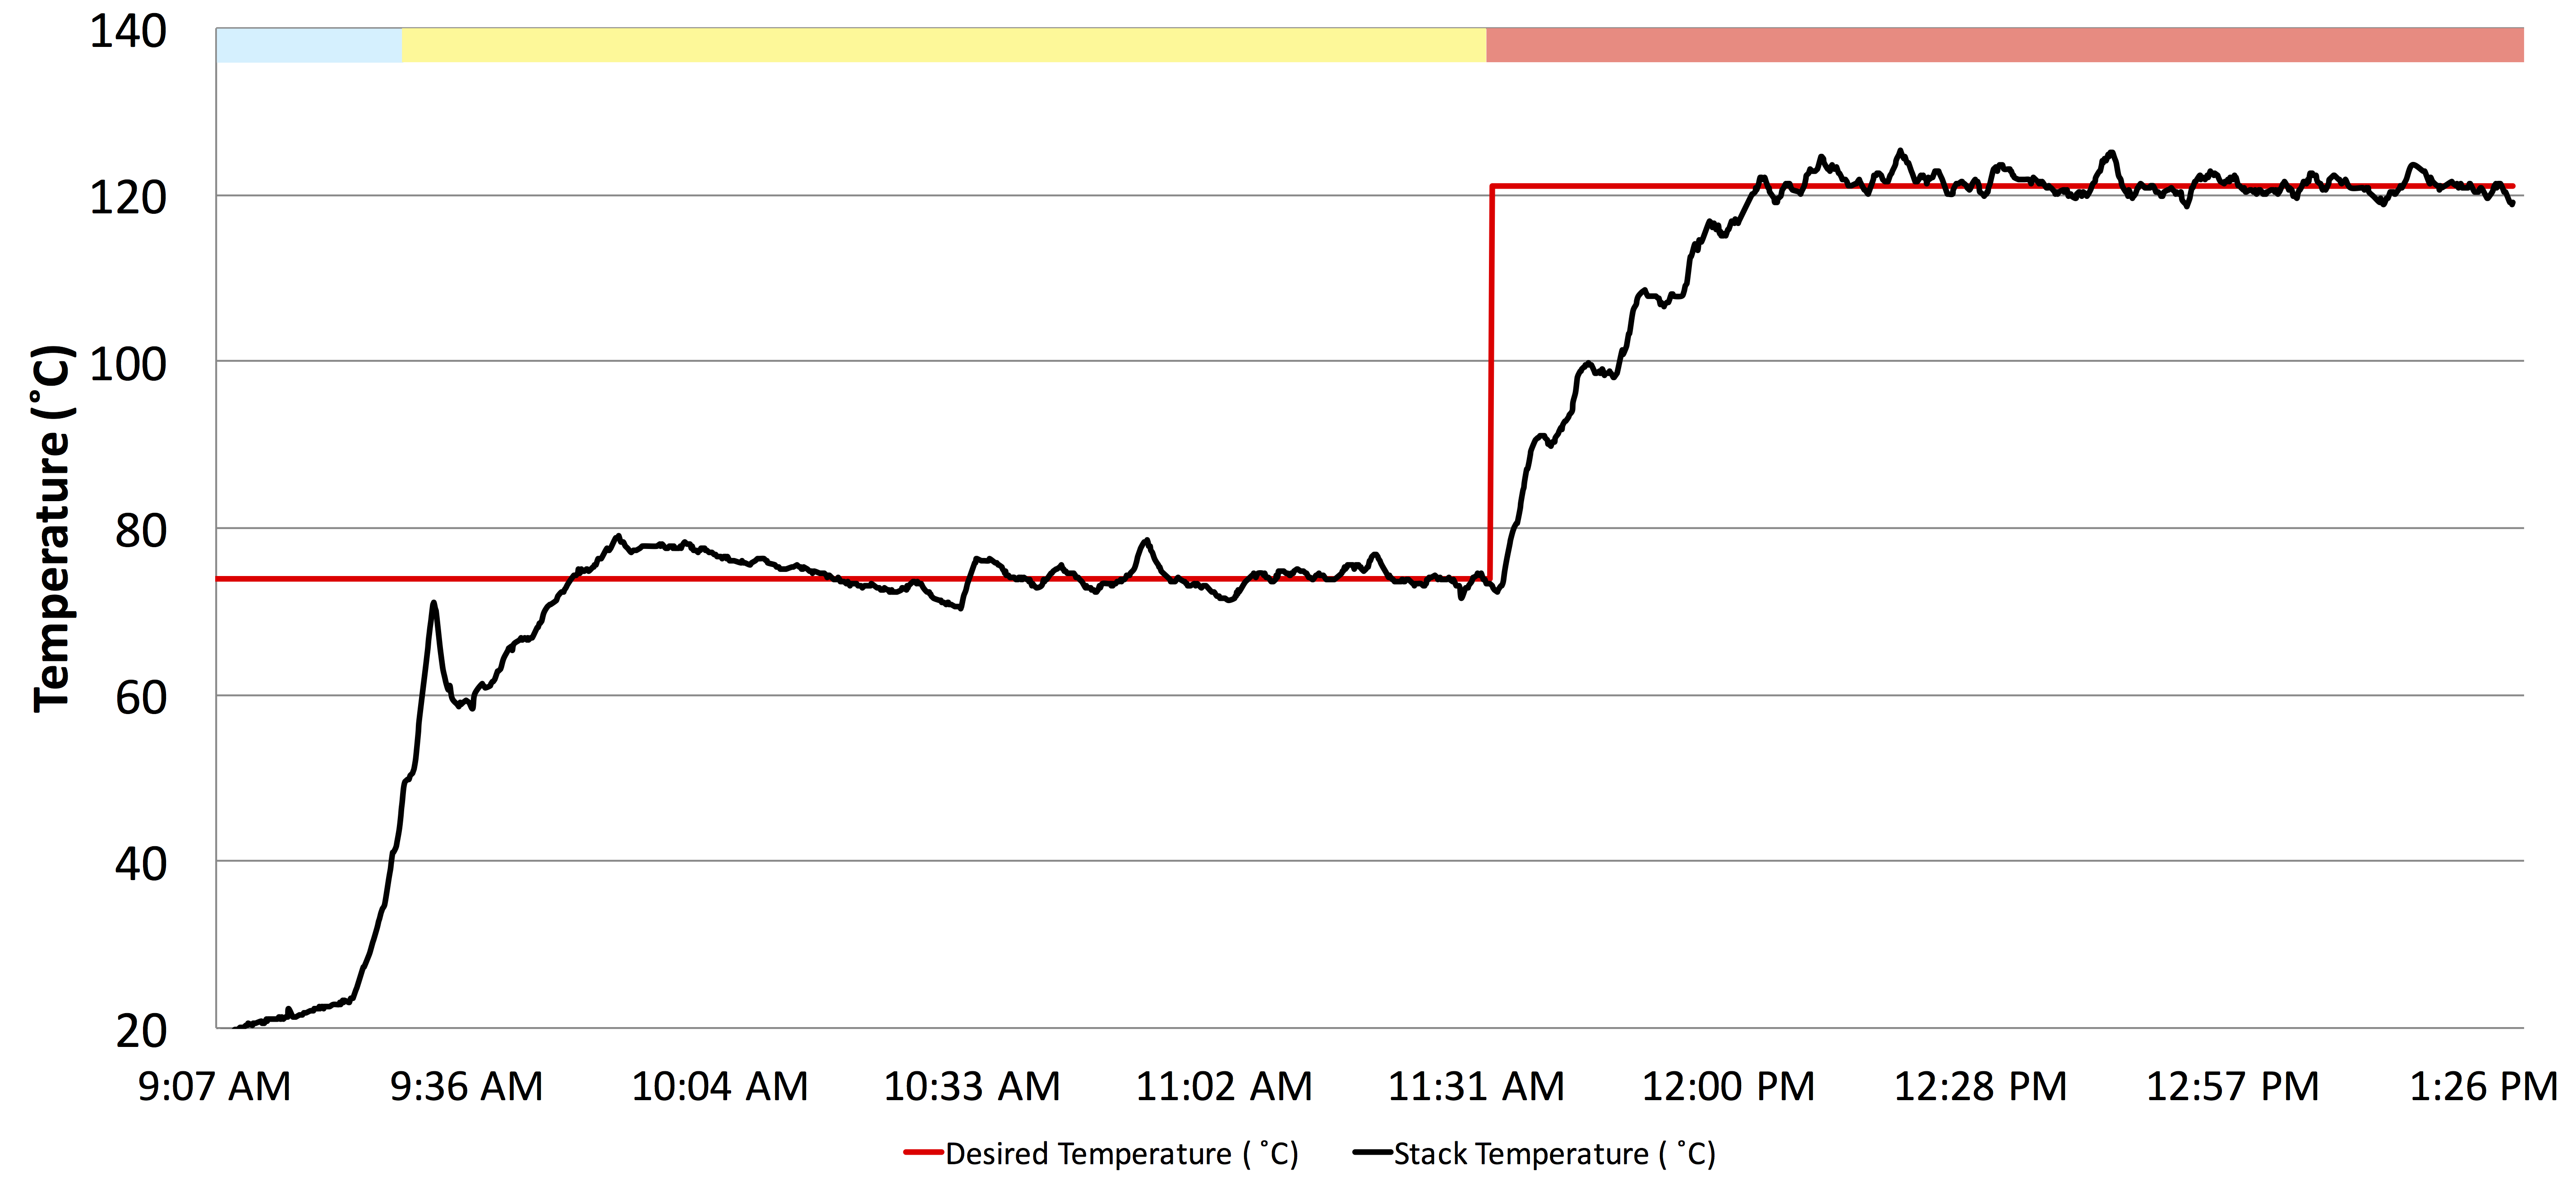
\includegraphics[scale=.3]{response2}
\centering
\end{center}
\textbf{FIG5.} Plot of start up (blue), smoke (yellow) and cook (red) state. 74\degree C set point in smoke state. 121\degree C set point in cook state.

\section{Firmware Configuration}
\begin{lstlisting}
#define FAN_PERIOD_LENGTH                       30
#define COLD_WARM_START_STACK_TRANSITION_TEMP   38      // 100 degF
#define MINIMUM_COOKING_TEMP                    76      // 170 degF
#define MINUTES                                 60      // its a minute. got it?
#define MINIMUM_FIRE_TEMP                       149     // 300 F
#define MAXIMUM_STARTUP_TIME                    3000    // 1500 seconds = 20 min
#define MAXIMUM_LOW_TEMP_COOK_TIME              600
#define MINIMUM_HOLD_TEMP                       60      //140F (meat cant be stored below this temp)
#define MINIMUM_STACK_TEMP                      71
#define START_UP_IGNITER_HEAT_UP_TIME           180     // 3 mins to initially heat up igniters
#define START_UP_INITIAL_AUGER_PERIOD           90
#define START_UP_INITIAL_AUGER_ON_TIME          30
uint16_t messagelength = 0;

volatile int16_t opState;
volatile uint8_t REBOOT = CLEAR;
volatile uint8_t manualControl = FALSE;
volatile uint8_t CONTROLLER_ENABLE = FALSE;


//PI controller settings
PIDController smokeTemperatureController; // only using PI control here,
                                          // adding derivative term could possibly reduce overshoot.
// kp = 6.005, thetap=2min, tp=33min, SM=3
volatile float CONTROLLER_GAIN = 0.83; // using Coheen-Coon 
volatile float CONTROLLER_INTEGRAL_TIME = 355.0; //using Coheen-Coon
volatile float CONTROLLER_DERIVATIVE_TIME = 0.0; //using Coheen-Coon
volatile float CONTROLLER_MIN_OUTPUT = 0.0; // 0 percent duty cycle controller min
volatile float CONTROLLER_MAX_OUTPUT = 12.0;  // 12 percent duty cycle max (prevent fire pots from overflowing)
volatile float INITIAL_CONTROLLER_OFFSET = 0.0; // multiply by Kc to get initial offset, ex: 15*0.3=4.5 = typical DLO CO

//State based setpoints
volatile float CONTROLLER_SAMPLING_PERIOD = 1.0; //sampling rate of 1 Hz
volatile float COOK_TEMPERATURE_SETPOINT = 121.0; //250F
volatile float HOLD_TEMPERATURE_SETPOINT = 73.0; //165F
volatile float SMOKE_TEMPERATURE_SETPOINT = 68.0; //155 F

//Start up settings
volatile float START_UP_AUGER_PERIOD = 100.0;
volatile float START_UP_FAN_DUTY_CYCLE = 100;
volatile int fireHasBeenPreviouslyDetected = FALSE;

//State based air:fuel ratios
volatile float COOK_STATE_AIR_TO_FUEL_SCALED_RATIO = 5.88;
volatile float SMOKE_STATE_AIR_TO_FUEL_SCALED_RATIO = 1.0;
volatile float HOLD_STATE_AIR_TO_FUEL_SCALED_RATIO = 5.88;

//State based auger on time for each pulse during PI controlled regions
volatile int8_t COOK_STATE_AUGER_ON_TIME = 2;
volatile int8_t SMOKE_STATE_AUGER_ON_TIME = 2;
volatile int8_t HOLD_STATE_AUGER_ON_TIME = 2;
\end{lstlisting}
\textbf{Code sample 1.} Current operation settings.
\end{document}








